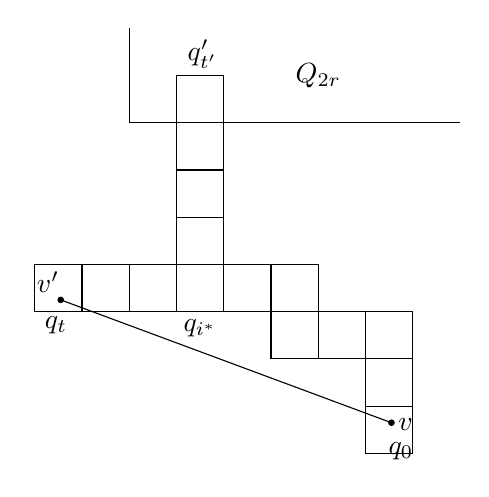
\begin{tikzpicture}[scale=0.6]
  % Unit squares forming the staircase/path
  \foreach \i/\j in {1/2,2/2,3/2,4/2,5/2,6/2, 6/1,7/1,8/1, 8/0,8/-1, 4/3,4/4,4/5,4/6} {
    \draw (\i,\j) -- ++(1,0) -- ++(0,1) -- ++(-1,0) -- cycle;
  }

  % Boundary indicating Q_{2r}
  \draw (3,8) -- (3,6) -- (10,6);
  \node at (7,7) {$Q_{2r}$};

  % Points v' and v with connecting segment
  \fill (1.55,2.25) circle (2pt);   % v' point
  \fill (8.55,-0.35) circle (2pt);  % v  point
  \draw (1.55,2.25) -- (8.55,-0.35);

  % Labels near the corresponding cells/points
  \node at (1.28,2.62) {$v'$};
  \node at (1.45,1.72) {$q_t$};

  \node at (8.75,-0.95) {$q_0$};
  \node at (8.85,-0.38) {$v$};

  \node at (4.50,1.65) {$q_{i^*}$};
  \node at (4.55,7.45) {$q'_{t'}$};
\end{tikzpicture}